\documentclass{standalone}
\usepackage{tikz}
\usetikzlibrary{patterns, positioning}


\begin{document}
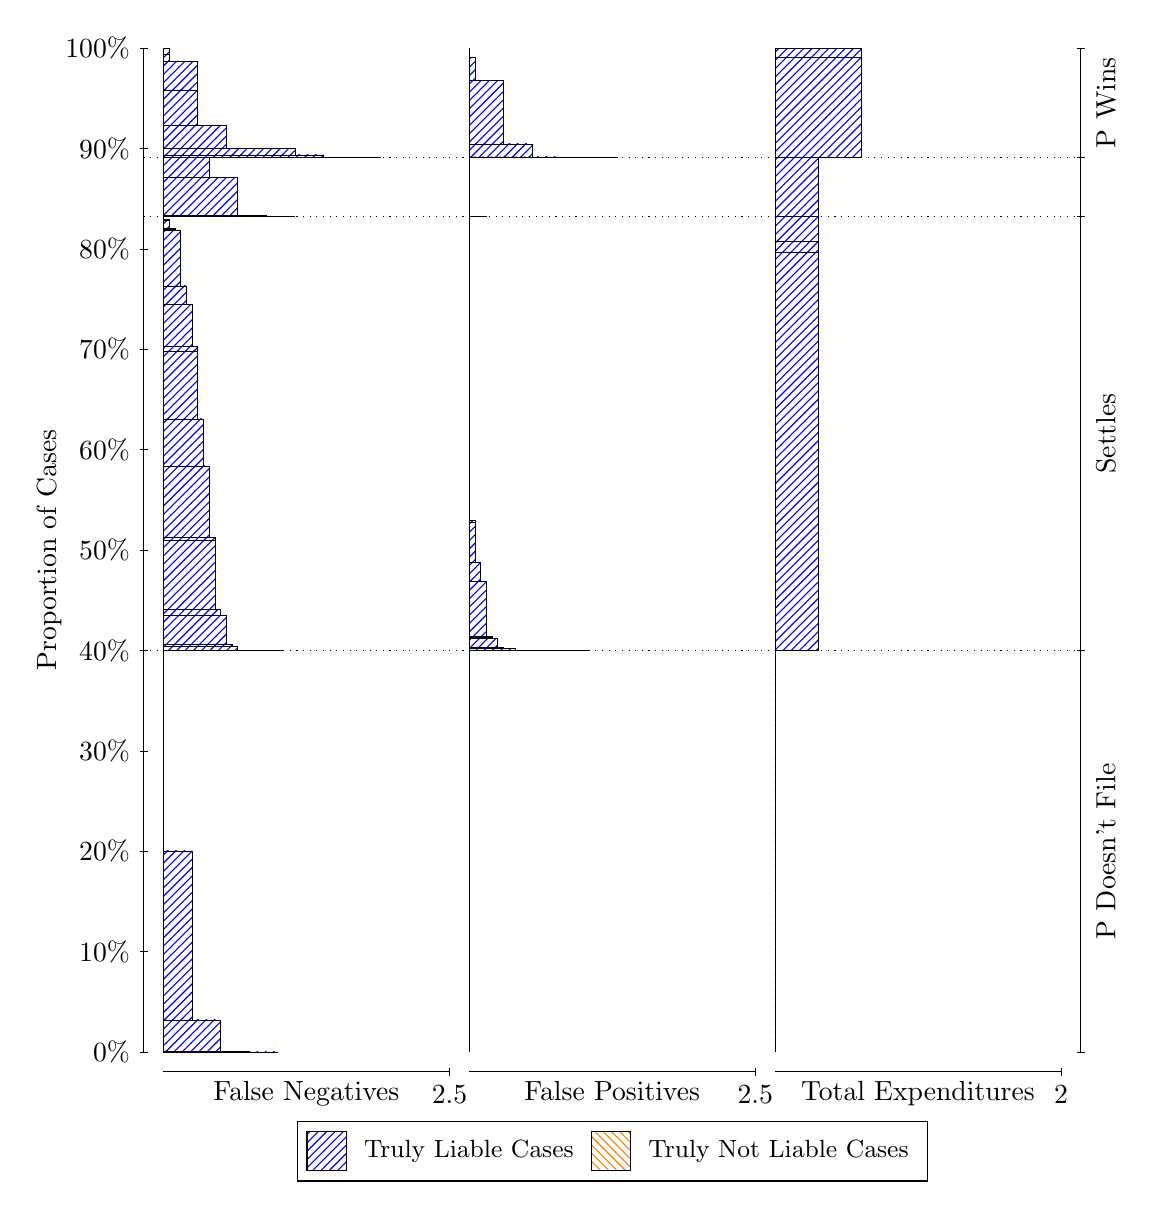
\begin{tikzpicture}
\draw[black, very thin] (1.5,1.75) -- (1.5,14.5);
\node[rotate=90, text=black, anchor=center] at (0.3, 8.125) {Proportion of Cases};
\draw[black, very thin] (1.45,1.75) -- (1.55,1.75);
\node[text=black, anchor=east] at (1.45, 1.75) {0\%};
\draw[black, very thin] (1.45,3.025) -- (1.55,3.025);
\node[text=black, anchor=east] at (1.45, 3.025) {10\%};
\draw[black, very thin] (1.45,4.3) -- (1.55,4.3);
\node[text=black, anchor=east] at (1.45, 4.3) {20\%};
\draw[black, very thin] (1.45,5.575) -- (1.55,5.575);
\node[text=black, anchor=east] at (1.45, 5.575) {30\%};
\draw[black, very thin] (1.45,6.85) -- (1.55,6.85);
\node[text=black, anchor=east] at (1.45, 6.85) {40\%};
\draw[black, very thin] (1.45,8.125) -- (1.55,8.125);
\node[text=black, anchor=east] at (1.45, 8.125) {50\%};
\draw[black, very thin] (1.45,9.4) -- (1.55,9.4);
\node[text=black, anchor=east] at (1.45, 9.4) {60\%};
\draw[black, very thin] (1.45,10.675) -- (1.55,10.675);
\node[text=black, anchor=east] at (1.45, 10.675) {70\%};
\draw[black, very thin] (1.45,11.95) -- (1.55,11.95);
\node[text=black, anchor=east] at (1.45, 11.95) {80\%};
\draw[black, very thin] (1.45,13.225) -- (1.55,13.225);
\node[text=black, anchor=east] at (1.45, 13.225) {90\%};
\draw[black, very thin] (1.45,14.5) -- (1.55,14.5);
\node[text=black, anchor=east] at (1.45, 14.5) {100\%};

\draw[black, very thin] (13.4,1.75) -- (13.4,14.5);
\draw[black, very thin] (13.35,1.75) -- (13.45,1.75);
\node[anchor=west] at (13.35, 1.75) {};
\draw[black, very thin] (13.35,6.8489) -- (13.45,6.8489);
\node[anchor=west] at (13.35, 6.8489) {};
\draw[black, very thin] (13.35,12.363) -- (13.45,12.363);
\node[anchor=west] at (13.35, 12.363) {};
\draw[black, very thin] (13.35,13.11) -- (13.45,13.11);
\node[anchor=west] at (13.35, 13.11) {};
\draw[black, very thin] (13.35,14.5) -- (13.45,14.5);
\node[anchor=west] at (13.35, 14.5) {};

\draw[black, very thin, pattern color=blue, pattern=north east lines] (1.75,1.75) rectangle (3.2033,1.75);
\draw[black, very thin, pattern color=blue, pattern=north east lines] (1.75,1.75) rectangle (2.84,1.7534);
\draw[black, very thin, pattern color=blue, pattern=north east lines] (1.75,1.7534) rectangle (2.4767,2.158);
\draw[black, very thin, pattern color=blue, pattern=north east lines] (1.75,2.158) rectangle (2.1133,4.3029);
\draw[black, very thin, pattern color=orange, pattern=north west lines] (1.75,4.3029) rectangle (1.75,4.3029);
\draw[black, very thin, pattern color=blue, pattern=north east lines] (1.75,4.3029) rectangle (1.75,6.8489);
\draw[black, very thin, pattern color=blue, pattern=north east lines] (1.75,6.8489) rectangle (3.276,6.8489);
\draw[black, very thin, pattern color=blue, pattern=north east lines] (1.75,6.8489) rectangle (3.1307,6.8489);
\draw[black, very thin, pattern color=blue, pattern=north east lines] (1.75,6.8489) rectangle (2.9853,6.8489);
\draw[black, very thin, pattern color=blue, pattern=north east lines] (1.75,6.8489) rectangle (2.9127,6.8513);
\draw[black, very thin, pattern color=blue, pattern=north east lines] (1.75,6.8513) rectangle (2.84,6.8518);
\draw[black, very thin, pattern color=blue, pattern=north east lines] (1.75,6.8518) rectangle (2.7673,6.8535);
\draw[black, very thin, pattern color=blue, pattern=north east lines] (1.75,6.8535) rectangle (2.6947,6.8996);
\draw[black, very thin, pattern color=blue, pattern=north east lines] (1.75,6.8996) rectangle (2.622,6.9303);
\draw[black, very thin, pattern color=blue, pattern=north east lines] (1.75,6.9303) rectangle (2.5493,7.2954);
\draw[black, very thin, pattern color=blue, pattern=north east lines] (1.75,7.2954) rectangle (2.4767,7.3741);
\draw[black, very thin, pattern color=blue, pattern=north east lines] (1.75,7.3741) rectangle (2.404,8.25);
\draw[black, very thin, pattern color=blue, pattern=north east lines] (1.75,8.25) rectangle (2.404,8.2813);
\draw[black, very thin, pattern color=blue, pattern=north east lines] (1.75,8.2813) rectangle (2.3313,9.1942);
\draw[black, very thin, pattern color=blue, pattern=north east lines] (1.75,9.1942) rectangle (2.2587,9.7893);
\draw[black, very thin, pattern color=blue, pattern=north east lines] (1.75,9.7893) rectangle (2.186,10.654);
\draw[black, very thin, pattern color=blue, pattern=north east lines] (1.75,10.654) rectangle (2.186,10.709);
\draw[black, very thin, pattern color=blue, pattern=north east lines] (1.75,10.709) rectangle (2.1133,11.248);
\draw[black, very thin, pattern color=blue, pattern=north east lines] (1.75,11.248) rectangle (2.0407,11.477);
\draw[black, very thin, pattern color=blue, pattern=north east lines] (1.75,11.477) rectangle (2.0407,11.479);
\draw[black, very thin, pattern color=blue, pattern=north east lines] (1.75,11.479) rectangle (1.968,12.186);
\draw[black, very thin, pattern color=blue, pattern=north east lines] (1.75,12.186) rectangle (1.8953,12.195);
\draw[black, very thin, pattern color=blue, pattern=north east lines] (1.75,12.195) rectangle (1.8953,12.21);
\draw[black, very thin, pattern color=blue, pattern=north east lines] (1.75,12.21) rectangle (1.8227,12.318);
\draw[black, very thin, pattern color=blue, pattern=north east lines] (1.75,12.318) rectangle (1.8227,12.319);
\draw[black, very thin, pattern color=blue, pattern=north east lines] (1.75,12.319) rectangle (1.75,12.319);
\draw[black, very thin, pattern color=orange, pattern=north west lines] (1.75,12.319) rectangle (1.75,12.319);
\draw[black, very thin, pattern color=blue, pattern=north east lines] (1.75,12.319) rectangle (1.75,12.363);
\draw[black, very thin, pattern color=blue, pattern=north east lines] (1.75,12.363) rectangle (3.4213,12.363);
\draw[black, very thin, pattern color=blue, pattern=north east lines] (1.75,12.363) rectangle (3.058,12.379);
\draw[black, very thin, pattern color=blue, pattern=north east lines] (1.75,12.379) rectangle (2.6947,12.86);
\draw[black, very thin, pattern color=blue, pattern=north east lines] (1.75,12.86) rectangle (2.3313,13.107);
\draw[black, very thin, pattern color=blue, pattern=north east lines] (1.75,13.107) rectangle (1.968,13.11);
\draw[black, very thin, pattern color=orange, pattern=north west lines] (1.75,13.11) rectangle (1.75,13.11);
\draw[black, very thin, pattern color=blue, pattern=north east lines] (1.75,13.11) rectangle (4.5113,13.11);
\draw[black, very thin, pattern color=blue, pattern=north east lines] (1.75,13.11) rectangle (4.148,13.11);
\draw[black, very thin, pattern color=blue, pattern=north east lines] (1.75,13.11) rectangle (3.7847,13.143);
\draw[black, very thin, pattern color=blue, pattern=north east lines] (1.75,13.143) rectangle (3.4213,13.227);
\draw[black, very thin, pattern color=blue, pattern=north east lines] (1.75,13.227) rectangle (3.276,13.227);
\draw[black, very thin, pattern color=blue, pattern=north east lines] (1.75,13.227) rectangle (3.058,13.229);
\draw[black, very thin, pattern color=blue, pattern=north east lines] (1.75,13.229) rectangle (2.9127,13.23);
\draw[black, very thin, pattern color=blue, pattern=north east lines] (1.75,13.23) rectangle (2.6947,13.23);
\draw[black, very thin, pattern color=blue, pattern=north east lines] (1.75,13.23) rectangle (2.5493,13.521);
\draw[black, very thin, pattern color=blue, pattern=north east lines] (1.75,13.521) rectangle (2.3313,13.521);
\draw[black, very thin, pattern color=blue, pattern=north east lines] (1.75,13.521) rectangle (2.186,13.969);
\draw[black, very thin, pattern color=blue, pattern=north east lines] (1.75,13.969) rectangle (2.186,14.326);
\draw[black, very thin, pattern color=blue, pattern=north east lines] (1.75,14.326) rectangle (1.8227,14.417);
\draw[black, very thin, pattern color=blue, pattern=north east lines] (1.75,14.417) rectangle (1.8227,14.493);
\draw[black, very thin, pattern color=orange, pattern=north west lines] (1.75,14.493) rectangle (1.75,14.493);
\draw[black, very thin, pattern color=blue, pattern=north east lines] (1.75,14.493) rectangle (1.75,14.5);
\draw[black, very thin, pattern color=orange, pattern=north west lines] (5.6333,1.75) rectangle (5.6333,1.75);
\draw[black, very thin, pattern color=blue, pattern=north east lines] (5.6333,1.75) rectangle (5.6333,6.8489);
\draw[black, very thin, pattern color=orange, pattern=north west lines] (5.6333,6.8489) rectangle (7.1593,6.8489);
\draw[black, very thin, pattern color=blue, pattern=north east lines] (5.6333,6.8489) rectangle (7.1593,6.8489);
\draw[black, very thin, pattern color=orange, pattern=north west lines] (5.6333,6.8489) rectangle (7.014,6.8489);
\draw[black, very thin, pattern color=blue, pattern=north east lines] (5.6333,6.8489) rectangle (7.014,6.8489);
\draw[black, very thin, pattern color=orange, pattern=north west lines] (5.6333,6.8489) rectangle (6.8687,6.8489);
\draw[black, very thin, pattern color=blue, pattern=north east lines] (5.6333,6.8489) rectangle (6.8687,6.8489);
\draw[black, very thin, pattern color=blue, pattern=north east lines] (5.6333,6.8489) rectangle (6.796,6.8489);
\draw[black, very thin, pattern color=orange, pattern=north west lines] (5.6333,6.8489) rectangle (6.7233,6.8489);
\draw[black, very thin, pattern color=blue, pattern=north east lines] (5.6333,6.8489) rectangle (6.7233,6.8489);
\draw[black, very thin, pattern color=blue, pattern=north east lines] (5.6333,6.8489) rectangle (6.6507,6.8489);
\draw[black, very thin, pattern color=orange, pattern=north west lines] (5.6333,6.8489) rectangle (6.578,6.8489);
\draw[black, very thin, pattern color=blue, pattern=north east lines] (5.6333,6.8489) rectangle (6.578,6.8489);
\draw[black, very thin, pattern color=blue, pattern=north east lines] (5.6333,6.8489) rectangle (6.5053,6.8489);
\draw[black, very thin, pattern color=orange, pattern=north west lines] (5.6333,6.8489) rectangle (6.4327,6.8489);
\draw[black, very thin, pattern color=blue, pattern=north east lines] (5.6333,6.8489) rectangle (6.4327,6.8489);
\draw[black, very thin, pattern color=orange, pattern=north west lines] (5.6333,6.8489) rectangle (6.4327,6.8489);
\draw[black, very thin, pattern color=blue, pattern=north east lines] (5.6333,6.8489) rectangle (6.4327,6.8489);
\draw[black, very thin, pattern color=blue, pattern=north east lines] (5.6333,6.8489) rectangle (6.36,6.849);
\draw[black, very thin, pattern color=blue, pattern=north east lines] (5.6333,6.849) rectangle (6.2873,6.849);
\draw[black, very thin, pattern color=orange, pattern=north west lines] (5.6333,6.849) rectangle (6.2873,6.849);
\draw[black, very thin, pattern color=blue, pattern=north east lines] (5.6333,6.849) rectangle (6.2873,6.849);
\draw[black, very thin, pattern color=blue, pattern=north east lines] (5.6333,6.849) rectangle (6.2147,6.8706);
\draw[black, very thin, pattern color=orange, pattern=north west lines] (5.6333,6.8706) rectangle (6.142,6.8706);
\draw[black, very thin, pattern color=blue, pattern=north east lines] (5.6333,6.8706) rectangle (6.142,6.8715);
\draw[black, very thin, pattern color=blue, pattern=north east lines] (5.6333,6.8715) rectangle (6.0693,6.8928);
\draw[black, very thin, pattern color=blue, pattern=north east lines] (5.6333,6.8928) rectangle (6.0693,6.8928);
\draw[black, very thin, pattern color=orange, pattern=north west lines] (5.6333,6.8928) rectangle (5.9967,6.8928);
\draw[black, very thin, pattern color=blue, pattern=north east lines] (5.6333,6.8928) rectangle (5.9967,7.0018);
\draw[black, very thin, pattern color=blue, pattern=north east lines] (5.6333,7.0018) rectangle (5.924,7.017);
\draw[black, very thin, pattern color=blue, pattern=north east lines] (5.6333,7.017) rectangle (5.924,7.0261);
\draw[black, very thin, pattern color=blue, pattern=north east lines] (5.6333,7.0261) rectangle (5.8513,7.7329);
\draw[black, very thin, pattern color=blue, pattern=north east lines] (5.6333,7.7329) rectangle (5.7787,7.9634);
\draw[black, very thin, pattern color=blue, pattern=north east lines] (5.6333,7.9634) rectangle (5.706,8.4806);
\draw[black, very thin, pattern color=blue, pattern=north east lines] (5.6333,8.4806) rectangle (5.706,8.5024);
\draw[black, very thin, pattern color=blue, pattern=north east lines] (5.6333,8.5024) rectangle (5.6333,12.363);
\draw[black, very thin, pattern color=orange, pattern=north west lines] (5.6333,12.363) rectangle (5.8513,12.363);
\draw[black, very thin, pattern color=blue, pattern=north east lines] (5.6333,12.363) rectangle (5.8513,12.366);
\draw[black, very thin, pattern color=blue, pattern=north east lines] (5.6333,12.366) rectangle (5.6333,13.11);
\draw[black, very thin, pattern color=orange, pattern=north west lines] (5.6333,13.11) rectangle (7.5227,13.11);
\draw[black, very thin, pattern color=blue, pattern=north east lines] (5.6333,13.11) rectangle (7.5227,13.11);
\draw[black, very thin, pattern color=orange, pattern=north west lines] (5.6333,13.11) rectangle (7.1593,13.11);
\draw[black, very thin, pattern color=blue, pattern=north east lines] (5.6333,13.11) rectangle (7.1593,13.11);
\draw[black, very thin, pattern color=orange, pattern=north west lines] (5.6333,13.11) rectangle (6.796,13.11);
\draw[black, very thin, pattern color=blue, pattern=north east lines] (5.6333,13.11) rectangle (6.796,13.117);
\draw[black, very thin, pattern color=orange, pattern=north west lines] (5.6333,13.117) rectangle (6.4327,13.117);
\draw[black, very thin, pattern color=blue, pattern=north east lines] (5.6333,13.117) rectangle (6.4327,13.283);
\draw[black, very thin, pattern color=blue, pattern=north east lines] (5.6333,13.283) rectangle (6.0693,14.089);
\draw[black, very thin, pattern color=orange, pattern=north west lines] (5.6333,14.089) rectangle (5.924,14.089);
\draw[black, very thin, pattern color=blue, pattern=north east lines] (5.6333,14.089) rectangle (5.924,14.089);
\draw[black, very thin, pattern color=blue, pattern=north east lines] (5.6333,14.089) rectangle (5.706,14.379);
\draw[black, very thin, pattern color=orange, pattern=north west lines] (5.6333,14.379) rectangle (5.6333,14.379);
\draw[black, very thin, pattern color=blue, pattern=north east lines] (5.6333,14.379) rectangle (5.6333,14.5);
\draw[black, very thin, pattern color=orange, pattern=north west lines] (9.5167,1.75) rectangle (9.5167,1.75);
\draw[black, very thin, pattern color=blue, pattern=north east lines] (9.5167,1.75) rectangle (9.5167,6.8489);
\draw[black, very thin, pattern color=orange, pattern=north west lines] (9.5167,6.8489) rectangle (10.062,6.8489);
\draw[black, very thin, pattern color=blue, pattern=north east lines] (9.5167,6.8489) rectangle (10.062,11.901);
\draw[black, very thin, pattern color=orange, pattern=north west lines] (9.5167,11.901) rectangle (10.062,11.901);
\draw[black, very thin, pattern color=blue, pattern=north east lines] (9.5167,11.901) rectangle (10.062,12.046);
\draw[black, very thin, pattern color=orange, pattern=north west lines] (9.5167,12.046) rectangle (10.062,12.046);
\draw[black, very thin, pattern color=blue, pattern=north east lines] (9.5167,12.046) rectangle (10.062,12.363);
\draw[black, very thin, pattern color=orange, pattern=north west lines] (9.5167,12.363) rectangle (10.062,12.363);
\draw[black, very thin, pattern color=blue, pattern=north east lines] (9.5167,12.363) rectangle (10.062,13.11);
\draw[black, very thin, pattern color=orange, pattern=north west lines] (9.5167,13.11) rectangle (10.607,13.11);
\draw[black, very thin, pattern color=blue, pattern=north east lines] (9.5167,13.11) rectangle (10.607,14.381);
\draw[black, very thin, pattern color=orange, pattern=north west lines] (9.5167,14.381) rectangle (10.607,14.381);
\draw[black, very thin, pattern color=blue, pattern=north east lines] (9.5167,14.381) rectangle (10.607,14.5);
\draw[black, dotted] (1.5,6.8489) -- (13.4,6.8489);
\draw[black, dotted] (1.5,12.363) -- (13.4,12.363);
\draw[black, dotted] (1.5,13.11) -- (13.4,13.11);
\draw[black, very thin] (1.75,1.5) -- (5.3833,1.5);
\node[text=black, anchor=north] at (3.5667, 1.5) {False Negatives};
\draw[black, very thin] (5.3833,1.45) -- (5.3833,1.55);
\node[text=black, anchor=north] at (5.3833, 1.45) {2.5};

\draw[black, very thin] (5.6333,1.5) -- (9.2667,1.5);
\node[text=black, anchor=north] at (7.45, 1.5) {False Positives};
\draw[black, very thin] (9.2667,1.45) -- (9.2667,1.55);
\node[text=black, anchor=north] at (9.2667, 1.45) {2.5};

\draw[black, very thin] (9.5167,1.5) -- (13.15,1.5);
\node[text=black, anchor=north] at (11.333, 1.5) {Total Expenditures};
\draw[black, very thin] (13.15,1.45) -- (13.15,1.55);
\node[text=black, anchor=north] at (13.15, 1.45) {2};

\node[text=black, centered, rotate=90] at (13.72, 4.2994) {P Doesn't File};
\node[text=black, centered, rotate=90] at (13.72, 9.6059) {Settles};

\node[text=black, centered, rotate=90] at (13.72, 13.805) {P Wins};

\draw (7.449999999999999,1.5) node[draw=none] (baseCoordinate) {};
\begin{scope}[align=center]
        \matrix[scale=0.5, draw=black, below=0.5cm of baseCoordinate, nodes={draw}, column sep=0.1cm]{
            \node[rectangle, draw, minimum width=0.5cm, minimum height=0.5cm, pattern color=blue, pattern=north east lines] {}; &
            \node[draw=none, font=\small, text=black] (B) {Truly Liable Cases}; &
            \node[rectangle, draw, minimum width=0.5cm, minimum height=0.5cm, pattern color=orange, pattern=north west lines] {}; &
            \node[draw=none, font=\small, text=black] (B) {Truly Not Liable Cases}; \\
            };
\end{scope}

\end{tikzpicture}
\end{document}